\documentclass{article}
    \title{\vspace{-50pt}\textbf{\underline{COP4620 Quiz 4 Work}}}
    \author{}
    \date{}
    \usepackage[T1]{fontenc}
    \usepackage{algorithm}
    \usepackage{algpseudocode}
	\usepackage{enumitem}
    \usepackage{makecell}
    \usepackage{multicol}
    \usepackage{pifont}
    \usepackage{soul}
    \usepackage{tikz}
    \usepackage{titlesec}
    \usepackage[tmargin=1in,lmargin=1in,rmargin=1in]{geometry}
    \usetikzlibrary{automata, positioning, arrows, babel,positioning,shapes}
    \tikzset{
        ->, % makes the edges directed
        >=stealth', % makes the arrow heads bold
        node distance=3cm, % minimum distance between two nodes. Change if necessary.
        every state/.style={thick, fill=gray!10}, % sets properties for each state node
        initial text=$ $, % sets the text that appears on the start arrow
    }
    \tikzset{
      gray box/.style={
		fill=gray!20,
		draw=gray,
		minimum width={2*#1ex},
		minimum height={2em},
	  },
  		annotation/.style={
    	anchor=north,
      }
  	}
    \tikzstyle{vertex}=[draw,fill=black!15,circle,minimum size=20pt,inner sep=0pt]
    
    \algdef{SE}{Begin}{End}{\textbf{begin}}{\textbf{end}}

    \newcommand{\cmark}{\ding{51}}%
    \newcommand{\xmark}{\ding{55}}%
    \newcommand{\textr}[1]{\textcolor{red}{#1}}

    \setlist[description]{noitemsep, topsep=0pt, itemsep=-.1em}
    \setlist[enumerate]{noitemsep, topsep=0pt, itemsep=-.1em}

    \newlength\tindent
    \setlength{\tindent}{\parindent}
    \setlength{\parindent}{0pt}
    \renewcommand{\indent}{\hspace*{\tindent}}

    \renewcommand{\familydefault}{\sfdefault}        	 
    \renewcommand\theadfont{\bfseries\sffamily}

	\titleformat{\chapter}[display]
	{\bfseries\Large\itshape}
	{Chapter\ \thechapter}{0.5ex}{ }

	\titleformat{\section}
	{\normalfont\bfseries}
	{\thesection}{0.5em}{}

	\titleformat{\subsection}
	{\normalfont\bfseries}
	{\thesubsection}{0.5em}{}
	
    \titlespacing\section{0pt}{12pt plus 4pt minus 8pt}{0pt plus 2pt minus 8pt}
    \titlespacing\subsection{0pt}{12pt plus 4pt minus 4pt}{0pt plus 2pt minus 4pt}

\begin{document}

\maketitle
\vspace{-60pt}

%\renewcommand\thechapter{Q1}
%\chapter{Take Home Quiz 4}

\section*{Question 2}
Consider the following attribute grammar.\newline

assign \hspace{.25em} $\rightarrow$ ID \textr{\#process\_id} := expr \textr{\#gen\_assign} \newline
expr \hspace{1em} $\rightarrow$ term addop term \textr{\#gen\_infix} \newline
term \hspace{.75em} $\rightarrow$ \textr{\#process\_id} | LIT \textr{\#process\_lit} \newline
addop \hspace{.2em} $\rightarrow$ + \textr{\#process\_p} | - \textr{\#process\_m} \newline

\begin{enumerate}[wide, labelwidth=!, labelindent=0pt]
  \item assign $\rightarrow$ ID \textr{\#process\_id} := \textbf{term addop term \textr{\#gen\_infix}} \textr{\#gen\_assign}
  \item assign $\rightarrow$ ID \textr{\#process\_id} := \textbf{LIT \textr{\#process\_lit}} addop \textbf{\textr{\#process\_id}} \textr{\#gen\_infix} \textr{\#gen\_assign}
  \item assign $\rightarrow$ ID \textr{\#process\_id} := LIT \textr{\#process\_lit} \textbf{+ \textr{\#process\_p}} \textr{\#process\_id} \textr{\#gen\_infix} \textr{\#gen\_assign}
\end{enumerate} \

Which sequence of actions are invoked for the string $a : = 1 + b$? 

\begin{enumerate}
  \item \textbf{\#process\_id}
  \item \textbf{\#process\_lit}
  \item \textbf{\#process\_p}
  \item \textbf{\#process\_id}
  \item \textbf{\#gen\_infix}
  \item \textbf{\#gen\_assign}
\end{enumerate}

\section*{Question 3}
Consider the following program:
\begin{algorithmic}[1]
  \Begin
    \State declare H, A, L: integer;
    \Begin
      \Begin
        \State declare X, Y: Real;
        \Begin
          \State declare A, C, M: char;
        \End;
      \End;
    \End;
  \End;
\end{algorithmic}
Apply the Symbol table generation algorithm discussed in the class and fill in the blanks.

Following is the status of the "Scope stack" after executing the line

\begin{multicols}{4}
\begin{center}
  \indent Line \textbf{2}\newline
  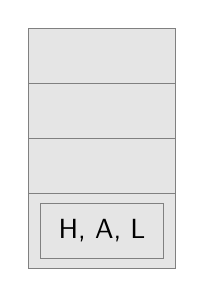
\begin{tikzpicture}[node distance=-0.5pt]
    \node [gray box=6] (0) {};
    \node [gray box=6, below=of 0] (1) {}; 
    \node [gray box=6, below=of 1] (2) {};
    \node [gray box=6, below=of 2] (3) {\tikz{\node[gray box=5] {H, A, L};}};
  \end{tikzpicture}
\end{center}
\columnbreak
\begin{center}
  \indent Line \textbf{5}\newline
  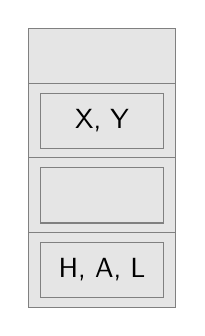
\begin{tikzpicture}[node distance=-0.5pt]
    \node [gray box=6] (0) {};
    \node [gray box=6, below=of 0] (1) {\tikz{\node[gray box=5] {X, Y};}}; 
    \node [gray box=6, below=of 1] (2) {\tikz{\node[gray box=5] {};}};
    \node [gray box=6, below=of 2] (3) {\tikz{\node[gray box=5] {H, A, L};}};
  \end{tikzpicture}
\end{center}
\columnbreak
\begin{center}
  \indent Line \textbf{7}\newline
  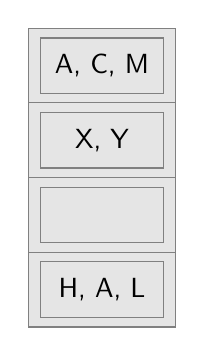
\begin{tikzpicture}[node distance=-0.5pt]
    \node [gray box=6] (0) {\tikz{\node[gray box=5] {A, C, M};}};
    \node [gray box=6, below=of 0] (1) {\tikz{\node[gray box=5] {X, Y};}}; 
    \node [gray box=6, below=of 1] (2) {\tikz{\node[gray box=5] {};}};
    \node [gray box=6, below=of 2] (3) {\tikz{\node[gray box=5] {H, A, L};}};
  \end{tikzpicture}
\end{center}
\columnbreak
\begin{center}
  \indent Line \textbf{9}\newline
  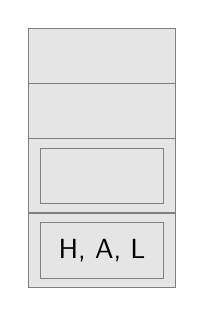
\begin{tikzpicture}[node distance=-0.5pt]
    \node [gray box=6] (0) {};
    \node [gray box=6, below=of 0] (1) {}; 
    \node [gray box=6, below=of 1] (2) {\tikz{\node[gray box=5] {};}};
    \node [gray box=6, below=of 2] (3) {\tikz{\node[gray box=5] {H, A, L};}};
  \end{tikzpicture}
\end{center}
\end{multicols}

\newpage
\section*{Question 4}
Consider the following program:
\begin{enumerate}
  \item int x;
  \item void f (int m)\{
  \item \indent float x, y;
  \item \indent \{
  \item \indent\indent int x, y;
  \item \indent \}
  \item \indent \{
  \item \indent\indent int x, I;
  \item \indent \}
  \item \}
  \item int g (int n)\{
  \item \indent bool t;
  \item \}
\end{enumerate}
Apply the Symbol table generation algorithm discussed in the class. Assume that function names are ignored (i.e. only variable declarations are included in the symbol tables).

Following is the status of the "Scope stack" after executing the line 

\begin{multicols}{4}
\begin{center}
  \indent Line \textbf{13}\newline
  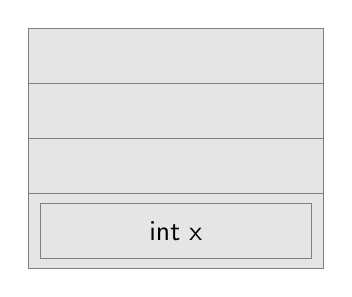
\begin{tikzpicture}[node distance=-0.5pt]
    \node [gray box=12] (0) {};
    \node [gray box=12, below=of 0] (1) {}; 
    \node [gray box=12, below=of 1] (2) {};
    \node [gray box=12, below=of 2] (3) {\tikz{\node[gray box=11] {int x};}};
  \end{tikzpicture}
\end{center}
\columnbreak
\begin{center}
  \indent Line \textbf{5}\newline
  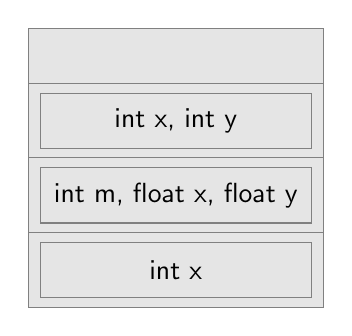
\begin{tikzpicture}[node distance=-0.5pt]
    \node [gray box=12] (0) {};
    \node [gray box=12, below=of 0] (1) {\tikz{\node[gray box=11] {int x, int y};}}; 
    \node [gray box=12, below=of 1] (2) {\tikz{\node[gray box=11] {int m, float x, float y};}};
    \node [gray box=12, below=of 2] (3) {\tikz{\node[gray box=11] {int x};}};
  \end{tikzpicture}
\end{center}
\columnbreak
\begin{center}
  \indent Line \textbf{8}\newline
  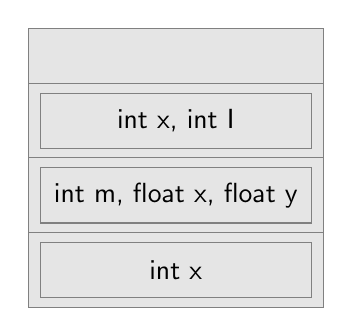
\begin{tikzpicture}[node distance=-0.5pt]
    \node [gray box=12] (0) {};
    \node [gray box=12, below=of 0] (1) {\tikz{\node[gray box=11] {int x, int I};}};
    \node [gray box=12, below=of 1] (2) {\tikz{\node[gray box=11] {int m, float x, float y};}};
    \node [gray box=12, below=of 2] (3) {\tikz{\node[gray box=11] {int x};}};
  \end{tikzpicture}
\end{center}
\columnbreak
\begin{center}
  \indent Line \textbf{12}\newline
  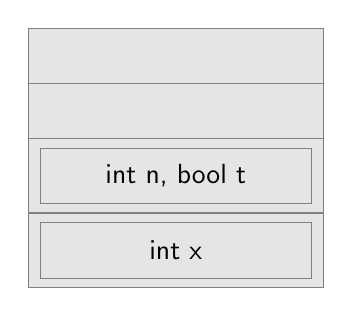
\begin{tikzpicture}[node distance=-0.5pt]
    \node [gray box=12] (0) {};
    \node [gray box=12, below=of 0] (1) {}; 
    \node [gray box=12, below=of 1] (2) {\tikz{\node[gray box=11] {int n, bool t};}};
    \node [gray box=12, below=of 2] (3) {\tikz{\node[gray box=11] {int x};}};
  \end{tikzpicture}
\end{center}
\end{multicols}

\section*{Question 5}
Consider the AST for the following: $x := y + z * w$ Assume typical operator precedence: \newline
https://mathworld.wolfram.com/Precedence.html \newline
\vspace{-1.5em}
\begin{multicols}{2}
  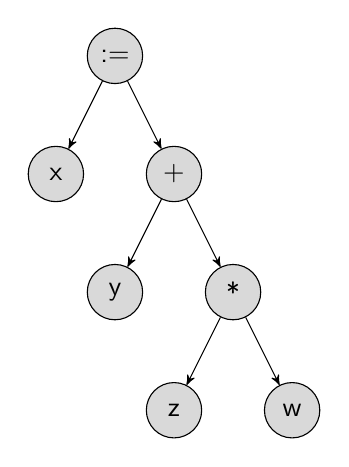
\begin{tikzpicture}
    \node[vertex]
    {:=}
        child {
            node[vertex] {x}
        } child {
            node[vertex] {+}
            child { node[vertex] {y} }
            child {
                node[vertex] {*}
                child { node[vertex] {z} }
                child { node[vertex] {w} }
            }
        }
    ;
  \end{tikzpicture}
  \begin{enumerate}
    \item The root node represents \textbf{:=}
    \item There are \textbf{7} nodes in the AST
    \item There are \textbf{4} leaf nodes, and they are \textbf{x, y, z, w}
  \end{enumerate}
\end{multicols}

\newpage
\section*{Question 6}
AST for: $(5 + z) / (- 8) * 4^2$ \newline
    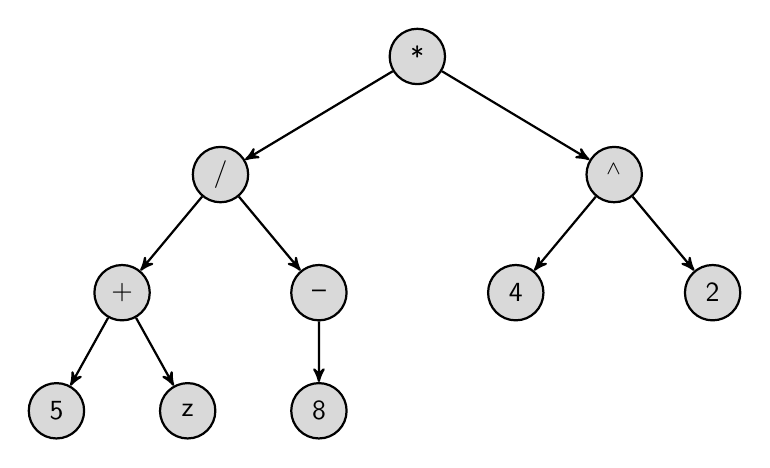
\begin{tikzpicture}[font=\sffamily,thick,level/.style={sibling distance=50mm/#1}]
    \node[vertex]
    {*}
        child {
            node[vertex] {/}
            child {
                node[vertex] {+}
                child { node[vertex] {5} }
                child { node[vertex] {z} }
            }
            child { 
                node[vertex] {--}
                child { node[vertex] {8} }
            }
        } child {
            node[vertex] {$^\wedge$}
            child { node[vertex] {4} }
            child { node[vertex] {2} }
        }
    ;
\end{tikzpicture} \newline
Post Order: \textbf{5, z, +, 8, --, /, 4, 2, $^\wedge$, *}

\section*{Question 7}
Select the correct statement(s).
\begin{description}
  \item [\cmark] A value that can appear on the left-hand side of an assignment statement should be labeled as an L-value.
  \item [\cmark] An address that can be stored to should be labeled as an L-value.
  \item [\cmark] A value that appears on the right-hand side of an assignment statement should be labeled as an R-value.
  \item [\cmark] Any "data" value should be defined as an R-value.
\end{description}


\section*{Question 8}
Select the correct statement(s).
\begin{description}
  \item [\cmark] The name of a temporary should be something that cannot appear in the program.
  \item [\xmark] \hspace{.25em}If the generated code includes temporaries, then the code is machine independent.
  \item [\cmark] Temporaries can be thought of as an unlimited pool of registers.
  \item [\cmark] Temporaries can hold either L-values or R-values.
\end{description}

\newpage
\section*{Question 9}
Consider the AST for the following: $x := y + z * w$ Assume typical operator precedence: \newline
https://mathworld.wolfram.com/Precedence.html \newline
\vspace{-1.5em}
\begin{multicols}{2}
  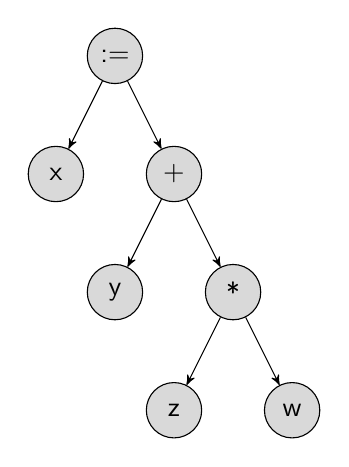
\begin{tikzpicture}
    \node[vertex]
    {:=}
        child {
            node[vertex] {x}
        } child {
            node[vertex] {+}
            child { node[vertex] {y} }
            child {
                node[vertex] {*}
                child { node[vertex] {z} }
                child { node[vertex] {w} }
            }
        }
    ;
  \end{tikzpicture}
  \begin{enumerate}[wide, labelwidth=!, labelindent=-1pt]
    \item How many AST nodes? \textbf{7}
    \item Which symbol is represented by the root node? \textbf{:=}
    \item How many data objects are flagged with L-values? \textbf{4}
    \item How many data objects are flagged with R-values? \textbf{2}
    \item How many data objects have code? \textbf{3}
  \end{enumerate}
  Post-order: \textbf{x, y, z, w, *, +, :=}
\end{multicols}
\section*{Question 10}
  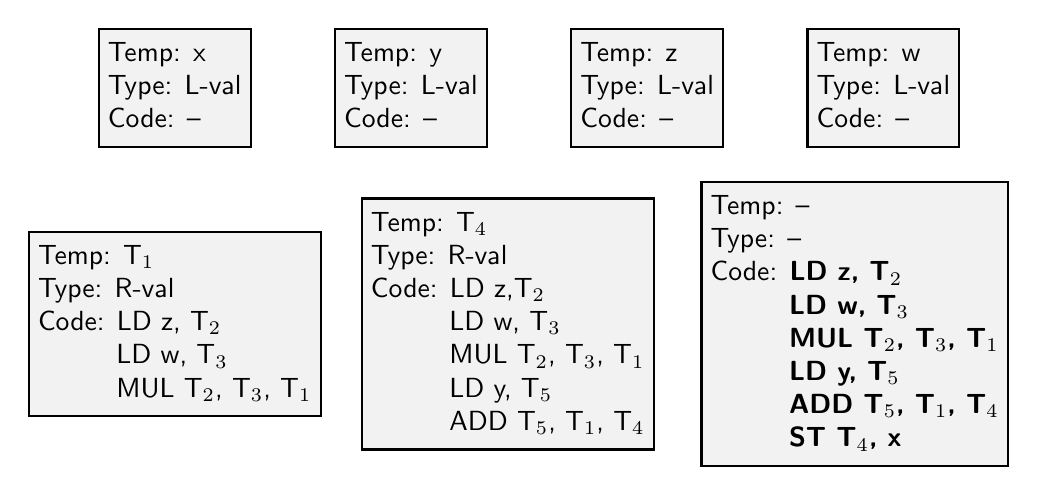
\begin{tikzpicture}
    \node[state, shape=rectangle] (0) {
    \makecell[l] {
    Temp: x \\
    Type: L-val \\
    Code: --
    }};
    \node[state, shape=rectangle, right of=0] (1) {
    \makecell[l] {
    Temp: y \\
    Type: L-val \\
    Code: --
    }};
    \node[state, shape=rectangle, right of=1] (2) {
    \makecell[l] {
    Temp: z \\
    Type: L-val \\
    Code: --
    }};
    \node[state, shape=rectangle, right of=2] (3) {
    \makecell[l] {
    Temp: w \\
    Type: L-val \\
    Code: --
    }};
    \node[state, shape=rectangle, below of=0] (4) {
    \makecell[l] {
    Temp: T$_1$ \\
    Type: R-val \\
    Code: LD z, T$_2$ \\
    \hspace{2.5em} LD w, T$_3$ \\
    \hspace{2.5em} MUL T$_2$, T$_3$, T$_1$
    }};
    \node[state, shape=rectangle, right of=4, xshift=35] (5) {
    \makecell[l] {
    Temp: T$_4$ \\
    Type: R-val \\
    Code: LD z,T$_2$ \\
    \hspace{2.5em} LD w, T$_3$ \\
    \hspace{2.5em} MUL T$_2$, T$_3$, T$_1$ \\
    \hspace{2.5em} LD y, T$_5$ \\
    \hspace{2.5em} ADD T$_5$, T$_1$, T$_4$
    }};
    \node[state, shape=rectangle, right of=5, xshift=40] (6) {
    \makecell[l] {
    Temp: -- \\
    Type: -- \\
    Code: \textbf{LD z, T$_2$} \\
    \hspace{2.5em} \textbf{LD w, T$_3$} \\
    \hspace{2.5em} \textbf{MUL T$_2$, T$_3$, T$_1$} \\
    \hspace{2.5em} \textbf{LD y, T$_5$} \\
    \hspace{2.5em} \textbf{ADD T$_5$, T$_1$, T$_4$} \\
    \hspace{2.5em} \textbf{ST T$_4$, x}
    }};
  \end{tikzpicture}

\section*{Question 11}
Consider the AST for the following: $x := (y + 3) * w$ Assume typical operator precedence: \newline
https://mathworld.wolfram.com/Precedence.html \newline
\vspace{-1.5em}
  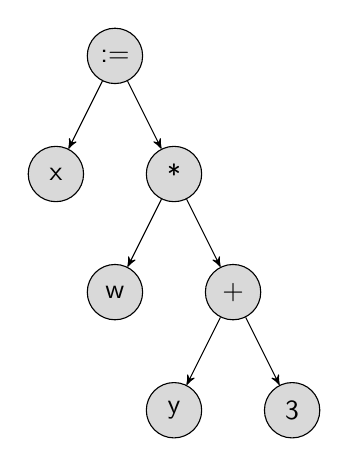
\begin{tikzpicture}
    \node[vertex]
    {:=}
        child {
            node[vertex] {x}
        } child {
            node[vertex] {*}
            child { node[vertex] {w} }
            child {
                node[vertex] {+}
                child { node[vertex] {y} }
                child { node[vertex] {3} }
            }
        }
    ;
  \end{tikzpicture}
  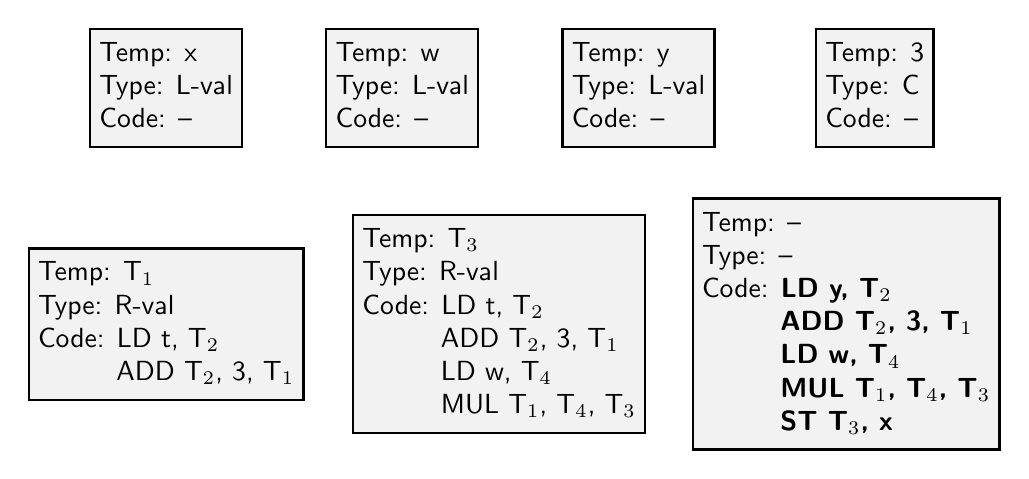
\begin{tikzpicture}
    \node[state, shape=rectangle] (0) {
    \makecell[l] {
    Temp: x \\
    Type: L-val \\
    Code: --
    }};
    \node[state, shape=rectangle, right of=0] (1) {
    \makecell[l] {
    Temp: w \\
    Type: L-val \\
    Code: --
    }};
    \node[state, shape=rectangle, right of=1] (2) {
    \makecell[l] {
    Temp: y \\
    Type: L-val \\
    Code: --
    }};
    \node[state, shape=rectangle, right of=2] (3) {
    \makecell[l] {
    Temp: 3 \\
    Type: C \\
    Code: --
    }};
    \node[state, shape=rectangle, below of=0] (4) {
    \makecell[l] {
    Temp: T$_1$ \\
    Type: R-val \\
    Code: LD t, T$_2$ \\
    \hspace{2.5em} ADD T$_2$, 3, T$_1$
    }};
    \node[state, shape=rectangle, right of=4, xshift=35] (5) {
    \makecell[l] {
    Temp: T$_3$ \\
    Type: R-val \\
    Code: LD t, T$_2$ \\
    \hspace{2.5em} ADD T$_2$, 3, T$_1$ \\
    \hspace{2.5em} LD w, T$_4$ \\
    \hspace{2.5em} MUL T$_1$, T$_4$, T$_3$
    }};
    \node[state, shape=rectangle, right of=5, xshift=40] (6) {
    \makecell[l] {
    Temp: -- \\
    Type: -- \\
    Code: \textbf{LD y, T$_2$} \\
    \hspace{2.5em} \textbf{ADD T$_2$, 3, T$_1$} \\
    \hspace{2.5em} \textbf{LD w, T$_4$} \\
    \hspace{2.5em} \textbf{MUL T$_1$, T$_4$, T$_3$} \\
    \hspace{2.5em} \textbf{ST T$_3$, x}
    }};
  \end{tikzpicture}\newline
  
  Post-order: \textbf{x, w, y, 3, +, *, :=}

\end{document}